\input{../preamble.tex}

\SetDate[27/05/2026]

\begin{document}
\pagestyle{fancy}
\fancyhead[L]{Seconde}
\fancyhead[C]{\textbf{Étude de variations}}
\fancyhead[R]{\today}


\exemulticols{}{
	Considérons la fonction $f$ donnée graphiquement ci-contre.
		\begin{enumerate}[itemsep=10pt] % pour Natalija
			\item Quel est le domaine de $f$ ? 
			\item Quel est le maximum de $f$ ?
			\item Quel est le minimum de $f$ ?
			\item Quels sont les zéros de $f$ ?
			\item Donner un candidat d'expression algébrique de $f$.
		\end{enumerate}
	\vfill\null
}{
	\begin{center}
	\begin{tikzpicture}[>=stealth, scale=1]
	\begin{axis}[xmin = -3, xmax=3, ymin=-1.5, ymax=5.5, y=25pt, axis x line=middle, axis y line=middle, axis line style=->, xlabel={}, ylabel={}, xtick distance = 1, ytick distance=1, grid=both]
		% (f)
		\addplot[BLUE_E, very thick, domain =-3:3, samples=50] {.5*(x+1)*(x-2)}  node[right] {$\C_f$};
		% trouvée par Thomas C.
	\end{axis}
	\end{tikzpicture}
	\end{center}
}{exe:aut0}{
		\begin{enumerate}
			\item
			$\D = [-3 ; 3]$.
			\item
			Le maximum de $f$ est environ 5 et il est atteint en $-3$. $f(-3) \approx 5$.
			\item 
			Le minimum de $f$ est environ $-1,2$ et il est atteint en $0,5$. $f(-0,5) \approx -1,2$.
			\item
			Les zéros de $f$ sont approximativement $-1$ et $2$ car $f(-1) = f(2) = 0$.
			\item 
			Une fonction qui s'annule en $-1$ et en $2$ est, par exemple, $F(x) = (x+1)(x-2)$.
			Cependant, $F(1) = 2 \times (-1) = -2$, alors que $f(1)$ semble être plutôt égal à $-1$.
			Dès lors, un meilleur candidat est plutôt $f(x) = \frac12 (x+1)(x-2)$ (et c'est la fonction graphée ici).
		\end{enumerate}
	\underline{Discussion}

	Le maximum et le minimum de $f$ sont atteints soit aux bornes du domaine, soit lorsque les variations de la fonction changent : elle passe de décroissante à croissante, ou de croissante à décroissante.
}

\exe{}{
	Remplir approximativement le tableau ci-dessous à l'aide des graphes de $\C_f$ et $\C_g$.
	
	\begin{center}
	\hspace{60pt}
	\begin{tikzpicture}[scale=1]
		\begin{axis}
			[xmin = -8, xmax=0, ymin=-4.3, ymax=3.5, axis x line=middle, axis y line=middle, axis line style=->, grid=both, ytick distance = 1, xtick distance=1, extra y ticks = {0},
			clip=false,
			x=45pt,
			y=15pt,
			every y tick label/.style={
			anchor=near yticklabel opposite,
			xshift=0.2em,
			}]
    			% (f)
			\addplot[no marks, myb, -, very thick] expression[domain=-8:-6, samples=2]{5*(x/2 + 3.2)}
			node[pos=0, left] {$\C_f$};
			\addplot[no marks, myb, -, very thick] expression[domain=-6:-3, samples=50]{(x+6)*(x+3)+1)};
			\addplot[no marks, myb, -, very thick] expression[domain=-3:0, samples=2]{5*0.2};
			
			% g sinus
			\addplot[no marks, myr, -, very thick] expression[domain=-8:0, samples=500]{2*sin(x*60)}
			node[pos=0, left]{$\C_g$};
		\end{axis}
	\end{tikzpicture}
	
	\hspace{-25pt}
	\begin{tikzpicture}[scale=1]
		\tkzTabInit
		 [lgt=3,espcl=2.1]
	       		{$x$ / 1 , Variation de $f(x)$ / 1.5, Variation de $g(x)$ / 1.5}
	       		{,,,,,,}
	\end{tikzpicture}
	\end{center}
}{exe:13}{
	\begin{center}
	\hspace{60pt}
	\begin{tikzpicture}[scale=1]
		\begin{axis}
			[xmin = -8, xmax=0, ymin=-4.3, ymax=3.5, axis x line=middle, axis y line=middle, axis line style=->, grid=both, ytick distance = 1, xtick distance=1, extra y ticks = {0},
			clip=false,
			x=45pt,
			y=15pt,
			every y tick label/.style={
			anchor=near yticklabel opposite,
			xshift=0.2em,
			}]
    			% (f)
			\addplot[no marks, myb, -, very thick] expression[domain=-8:-6, samples=2]{5*(x/2 + 3.2)}
			node[pos=0, left] {$\C_f$};
			\addplot[no marks, myb, -, very thick] expression[domain=-6:-3, samples=50]{(x+6)*(x+3)+1)};
			\addplot[no marks, myb, -, very thick] expression[domain=-3:0, samples=2]{5*0.2};
			
			% g sinus
			\addplot[no marks, myr, -, very thick] expression[domain=-8:0, samples=500]{2*sin(x*60)}
			node[pos=0, left]{$\C_g$};
		\end{axis}
	\end{tikzpicture}
	
	\hspace{-25pt}
	\begin{tikzpicture}[scale=1]
		\tkzTabInit
		 [lgt=3,espcl=2.1]
	       		{$x$ / 1 , Variation de $f(x)$ / 1.5, Variation de $g(x)$ / 1.5}
	       		{ $-8$ , ${-7,5}$ , {$-6$} , {$-4,5$} ,  {$-3$} ,  {$-1,5$} ,  {$0$} }
		\tkzTabVar
			{-/{$-4$},R/ ,+/{$1$}, -/{$1,2$}, +/{$1$}, R/, +/{$1$}}
	       	
		\tkzTabVar
			{+/{$-1,8$},-/{$-2$},R/,+/{$2$},R/,-/{$-2$},+/{$0$}}
	\end{tikzpicture}
	\end{center}

}

\exe{,difficulty=1}{
	Pour chaque proposition suivante, dire si elle est \underline{toujours vraie} ou si elle \underline{peut être fausse} à l'aide du tableau de variations suivant.
	
	\begin{center}
	\begin{tikzpicture}[scale=1]
		\tkzTabInit
		 [lgt=3,espcl=2]
	       		{$x$ / 1 , Variation de $f(x)$ / 1.5}
	       		{7,$a$,11,$b$,$c$,28,$d$,31}
			
		\tkzTabVar
			{-/, +/,-/$-45$,R/,R/,+/$20$, R/, -/{$-30$}}
		\tkzTabIma
			{1}{2}{1}{$30$}
	\end{tikzpicture}

	\vfill\null

\def\arraystretch{1.5}
\setlength\tabcolsep{6pt}
	\begin{tabular}{|c|c|c|} \hline
		Proposition & Vrai & Faux \\ \hline
		$f(a) = 35$ & &  \\ \hline
		$f(a) > 30$ &  & \\ \hline
		$f(b) \leq 20$ &  & \\ \hline
		$f(a) > f(b)$ &  & \\ \hline
	\end{tabular}	
	\hfill
	\begin{tabular}{|c|c|c|} \hline
		Proposition & Vrai & Faux \\ \hline
		$f(b) < f(c)$ &  & \\ \hline
		$f(c) < f(a)$ &  & \\ \hline
		$f(c) = 19$ & &  \\ \hline
		$f(c) < 30$ &  & \\ \hline
	\end{tabular}
	\hfill
	\begin{tabular}{|c|c|c|} \hline
		Proposition & Vrai & Faux \\ \hline
		$f(d) = -5$ & &  \\ \hline
		$f(d) < 0$ & &  \\ \hline
		$f(c) = f(d)$ & &  \\ \hline
		$f(d) \geq -30$ &  & \\ \hline
	\end{tabular}	
	\end{center}

}{exe:16}{

	\begin{center}
\def\arraystretch{1.5}
\setlength\tabcolsep{6pt}
	\begin{tabular}{|c|c|c|} \hline
		Proposition & Vrai & Faux \\ \hline
		$f(a) = 35$ & & \checkmark \\ \hline
		$f(a) > 30$ & \checkmark & \\ \hline
		$f(b) \leq 20$ & \checkmark & \\ \hline
		$f(a) > f(b)$ & \checkmark & \\ \hline
	\end{tabular}	
	\hfill
	\begin{tabular}{|c|c|c|} \hline
		Proposition & Vrai & Faux \\ \hline
		$f(b) < f(c)$ & \checkmark & \\ \hline
		$f(c) < f(a)$ & \checkmark & \\ \hline
		$f(c) = 19$ & & \checkmark \\ \hline
		$f(c) < 30$ & \checkmark & \\ \hline
	\end{tabular}
	\hfill
	\begin{tabular}{|c|c|c|} \hline
		Proposition & Vrai & Faux \\ \hline
		$f(d) = -5$ & & \checkmark \\ \hline
		$f(d) < 0$ & & \checkmark \\ \hline
		$f(c) = f(d)$ & & \checkmark \\ \hline
		$f(d) \geq -30$ & \checkmark & \\ \hline
	\end{tabular}	
	\end{center}
}

\begin{multicols}{2}
\begin{Exercise}[label=exe:10]
	Tracer la droite $y=3x - 2$ et remplir le tableau de variations ci-dessous.
	
	\begin{center}
	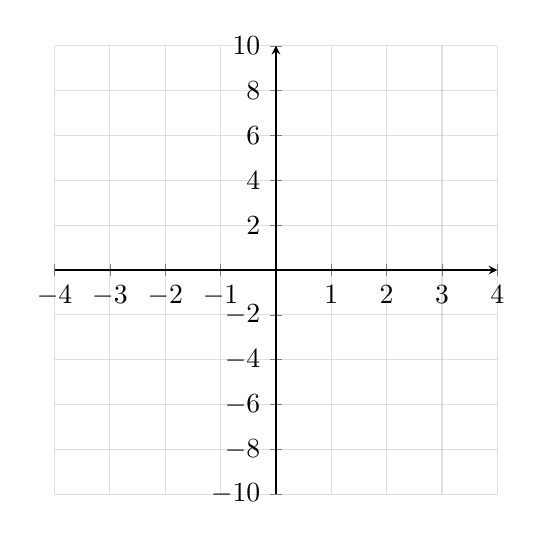
\begin{tikzpicture}[>=stealth]
		\begin{axis}[xmin = -4, xmax=4, ymin=-10, ymax=10, axis x line=middle, axis y line=middle, axis line style=->, grid=both,
			grid style = {opacity=.5},
			x=20pt,
			xtick distance=1,
			ytick distance=2,
			%y=20pt,
			clip=true,
			]
			\addplot[no marks, transparent, -, very thick] expression[domain=-4:4, samples=2]{3*x-2}
			node[left, pos=.9]{$y=3x-2$};
		\end{axis}
	\end{tikzpicture}
	
	\hspace{-55pt}
	\begin{tikzpicture}
		\tkzTabInit
		[lgt=2,espcl=2.6]
	       		{$x$ / 1, Variation de $3x-2$ / 1.5}
			{,,}
	\end{tikzpicture}
	\end{center}
\end{Exercise}

\columnbreak

\begin{Exercise}[label=exe:11]
	Tracer la droite $y = -6x - 2$ et remplir le tableau de variations ci-dessous.
	
	\begin{center}
	\hspace{55pt}
	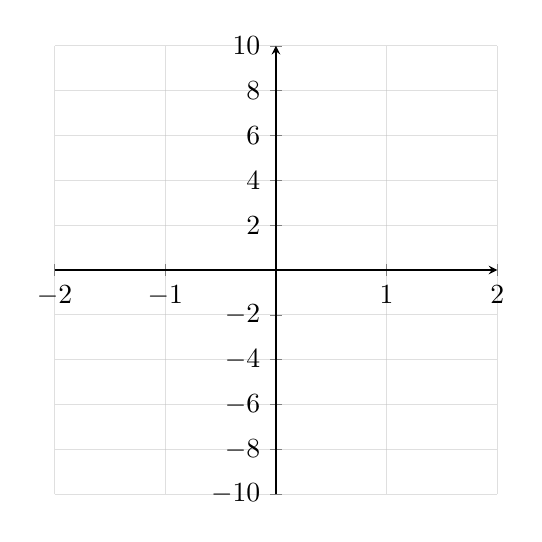
\begin{tikzpicture}[>=stealth]
		\begin{axis}[xmin = -2, xmax=2, ymin=-10, ymax=10, axis x line=middle, axis y line=middle, axis line style=->, grid=both,
			grid style = {opacity=.5},
			x=40pt,
			xtick distance=1,
			ytick distance=2,
			%y=20pt,
			clip=true,
			]
			\addplot[no marks, transparent, -, very thick] expression[domain=-2:2, samples=2]{-6*x-2}
			node[right, pos=.55]{$y=-6x-2$};
		\end{axis}
	\end{tikzpicture}
	
	\begin{tikzpicture}
		\tkzTabInit
		[lgt=2.2,espcl=2.7]
	       		{$x$ / 1 , Variation \mbox{de $-6x-2$} / 1.5}
			{,,}
	\end{tikzpicture}
	\end{center}
\end{Exercise}

\end{multicols}


\begin{Answer}[ref=exe:10]
	\begin{center}
	\begin{tikzpicture}[>=stealth]
		\begin{axis}[xmin = -4, xmax=4, ymin=-10, ymax=10, axis x line=middle, axis y line=middle, axis line style=->, grid=both,
			grid style = {opacity=.5},
			x=20pt,
			xtick distance=1,
			ytick distance=2,
			%y=20pt,
			clip=true,
			]
			\addplot[no marks, BLUE_E, -, very thick] expression[domain=-4:4, samples=2]{3*x-2}
			node[left, pos=.9]{$y=3x-2$};
		\end{axis}
	\end{tikzpicture}
	
	\begin{tikzpicture}
		\tkzTabInit
		 %[lgt=3,espcl=1.5]
	       		{$x$ / 1 , Variation de $3x-2$ / 2}
	       		{  $-4$ ,,  $\dfrac23$ ,,  $4$ }
	       	
		\tkzTabVar
			{-/$-14$, R/, R/, R/, +/$10$}
		\tkzTabIma
			{1}{5}{3}{0}
	\end{tikzpicture}
	\end{center}
\end{Answer}

\begin{Answer}[ref=exe:11]
	\begin{center}
	\begin{tikzpicture}[>=stealth]
		\begin{axis}[xmin = -2, xmax=2, ymin=-10, ymax=10, axis x line=middle, axis y line=middle, axis line style=->, grid=both,
			grid style = {opacity=.5},
			x=40pt,
			xtick distance=1,
			ytick distance=2,
			clip=true,
			]
			\addplot[no marks, BLUE_E, -, very thick] expression[domain=-2:2, samples=2]{-6*x-2}
			node[right, pos=.55]{$y=-6x-2$};
		\end{axis}
	\end{tikzpicture}
	
	\begin{tikzpicture}
		\tkzTabInit
		 %[lgt=3,espcl=1.5]
	       		{$x$ / 1 , Variation de $-6x-2$ / 2}
	       		{  $-2$ ,,  $-\dfrac13$ ,,  $2$ }
	       	
		\tkzTabVar
			{+/$10$, R/, R/, R/, -/$-14$}
		\tkzTabIma
			{1}{5}{3}{0}
	\end{tikzpicture}
	\end{center}
\end{Answer}


\exe{,difficulty=1}{
	Considérons la courbe $\C_f$ graphiquement ci-dessous. 
	Dans les deux repères, tracer la courbe représentative de chaque fonction suivante puis remplir son tableau de variations.
		\begin{multicols}{4}
		\begin{enumerate}[label=]
			\item $g(x) = f(x) + 1$
			\item $h(x) = f(x) - 2$
			\item $k(x) = 2f(x)$
			\item $\ell(x) = -f(x)$
		\end{enumerate}
		\end{multicols}
	
%	\begin{enumerate}
%		\item Esquisser, dans le même repère, la courbe de $g(x) = f(x)+1$.
%		\item Esquisser, dans le même repère, la courbe de $h(x) = f(x)-2$.
%		\item Remplir le tableau de variations ci-dessous.
%	\end{enumerate}
%	
	\begin{multicols}{2}
	\hspace{-50pt}
	\begin{tikzpicture}[scale=1]
		\begin{axis}[xmin = -10, xmax=7, ymin=-4.25, ymax=3.25, axis x line=middle, axis y line=middle, axis line style=->, grid=both,
		x=15pt,
		y=20pt,
		ytick distance=1,
		xtick distance=2,
		clip=false,
	    	]
		\addplot[no marks, myb, -, very thick] expression[domain=-10:7, samples=50]{.01*(x+6)*(x+3)*(x-5)}
		node[pos=0, left]{$\mathcal{C}_f$};
		\end{axis}
	\end{tikzpicture}
	
	\begin{tikzpicture}
		\tkzTabInit
		 [espcl=2]
	       		{$x$ / 1 , Variation de $f(x)$ / 1.5, Variation de $g(x)$ / 1.5, Variation de $h(x)$ / 1.5}
	       		{$-10$,,,$7$}
	\end{tikzpicture}
	\end{multicols}

	\begin{multicols}{2}
	\hspace{-50pt}
	\begin{tikzpicture}[scale=1]
		\begin{axis}[xmin = -10, xmax=7, ymin=-4.25, ymax=3.25, axis x line=middle, axis y line=middle, axis line style=->, grid=both,
		x=15pt,
		y=20pt,
		ytick distance=1,
		xtick distance=2,
		clip=false,
	    	]
		\addplot[no marks, myb, -, very thick] expression[domain=-10:7, samples=50]{.01*(x+6)*(x+3)*(x-5)}
		node[pos=0, left]{$\mathcal{C}_f$};
		\end{axis}
	\end{tikzpicture}
	
	\begin{tikzpicture}
		\tkzTabInit
		 [espcl=2]
	       		{$x$ / 1 , Variation de $f(x)$ / 1.5, Variation de $k(x)$ / 1.5, Variation de $\ell(x)$ / 1.5}
	       		{$-10$,,,$7$}
	\end{tikzpicture}
	\end{multicols}

}{exe:parentes1}{
	\begin{multicols}{2}
	\hspace{-60pt}
	\begin{tikzpicture}[scale=1]
		\begin{axis}[xmin = -10, xmax=7, ymin=-6.25, ymax=3.75, axis x line=middle, axis y line=middle, axis line style=->, grid=both,
		x=15pt,
		y=20pt,
		ytick distance=1,
		xtick distance=2,
		clip=false,
	    	]
		\addplot[no marks, myb, -, very thick] expression[domain=-10:7, samples=50]{.01*(x+6)*(x+3)*(x-5)}
		node[pos=0, left]{$\mathcal{C}_f$};
		\addplot[no marks, myr, -, very thick] expression[domain=-10:7, samples=50]{.01*(x+6)*(x+3)*(x-5)+1}
		node[pos=0, left]{$\mathcal{C}_g$};
		\addplot[no marks, myg, -, very thick] expression[domain=-10:7, samples=50]{.01*(x+6)*(x+3)*(x-5)-2}
		node[pos=0, left]{$\mathcal{C}_h$};
		\end{axis}
	\end{tikzpicture}
	\begin{tikzpicture}
		\tkzTabInit
		 [espcl=2]
	       		{$x$ / 1 , Variation de $f(x)$ / 2, Variation de $g(x)$ / 2, Variation de $h(x)$ / 2}
	       		{$-10$,{$-4,6$}, {2},$7$}
	       	
		\tkzTabVar
			{-/{$-4,1$}, +/{$0,2$}, -/{$-1,2$}, +/{$2,5$}}
		\tkzTabVar
			{-/{$-3,1$}, +/{$1,2$}, -/{$-0,2$}, +/{$3,5$}}
		\tkzTabVar
			{-/{$-6,1$}, +/{$-1,8$}, -/{$-3,2$}, +/{$0,5$}}
	\end{tikzpicture}
	\end{multicols}


	\begin{multicols}{2}
	\hspace{-60pt}
	\begin{tikzpicture}[scale=1]
		\begin{axis}[xmin = -10, xmax=7, ymin=-8.5, ymax=5.25, axis x line=middle, axis y line=middle, axis line style=->, grid=both,
		x=15pt,
		y=20pt,
		ytick distance=1,
		xtick distance=2,
		clip=false,
	    	]
		\addplot[no marks, myb, -, very thick] expression[domain=-10:7, samples=50]{.01*(x+6)*(x+3)*(x-5)}
		node[pos=0, left]{$\mathcal{C}_f$};
		\addplot[no marks, myr, -, very thick] expression[domain=-10:7, samples=50]{.02*(x+6)*(x+3)*(x-5)}
		node[pos=0, left]{$\mathcal{C}_k$};
		\addplot[no marks, myg, -, very thick] expression[domain=-10:7, samples=50]{-.01*(x+6)*(x+3)*(x-5)}
		node[pos=0, left]{$\mathcal{C}_\ell$};
		\end{axis}
	\end{tikzpicture}
	\begin{tikzpicture}
		\tkzTabInit
		 [espcl=2]
	       		{$x$ / 1 , Variation de $f(x)$ / 2, Variation de $k(x)$ / 2, Variation de $\ell(x)$ / 2}
	       		{$-10$,{$-4,6$}, {2},$7$}
	       	
		\tkzTabVar
			{-/{$-4,1$}, +/{$0,2$}, -/{$-1,2$}, +/{$2,5$}}
		\tkzTabVar
			{-/{$-8,2$}, +/{$0,4$}, -/{$-2,4$}, +/{$5$}}
		\tkzTabVar
			{+/{$4,1$}, -/{$-0,2$}, +/{$1,2$}, -/{$-2,5$}}
	\end{tikzpicture}
	\end{multicols}
}

%%%%%%%%%%%

\newpage
\fancyhead[C]{\textbf{Solutions}}
\shipoutAnswer

\end{document}
